\documentclass[11pt,compress,t,notes=noshow, xcolor=table]{beamer}
\usepackage[]{graphicx}\usepackage[]{color}
% maxwidth is the original width if it is less than linewidth
% otherwise use linewidth (to make sure the graphics do not exceed the margin)
\makeatletter
\def\maxwidth{ %
  \ifdim\Gin@nat@width>\linewidth
    \linewidth
  \else
    \Gin@nat@width
  \fi
}
\makeatother

\definecolor{fgcolor}{rgb}{0.345, 0.345, 0.345}
\newcommand{\hlnum}[1]{\textcolor[rgb]{0.686,0.059,0.569}{#1}}%
\newcommand{\hlstr}[1]{\textcolor[rgb]{0.192,0.494,0.8}{#1}}%
\newcommand{\hlcom}[1]{\textcolor[rgb]{0.678,0.584,0.686}{\textit{#1}}}%
\newcommand{\hlopt}[1]{\textcolor[rgb]{0,0,0}{#1}}%
\newcommand{\hlstd}[1]{\textcolor[rgb]{0.345,0.345,0.345}{#1}}%
\newcommand{\hlkwa}[1]{\textcolor[rgb]{0.161,0.373,0.58}{\textbf{#1}}}%
\newcommand{\hlkwb}[1]{\textcolor[rgb]{0.69,0.353,0.396}{#1}}%
\newcommand{\hlkwc}[1]{\textcolor[rgb]{0.333,0.667,0.333}{#1}}%
\newcommand{\hlkwd}[1]{\textcolor[rgb]{0.737,0.353,0.396}{\textbf{#1}}}%
\let\hlipl\hlkwb

\usepackage{framed}
\makeatletter
\newenvironment{kframe}{%
 \def\at@end@of@kframe{}%
 \ifinner\ifhmode%
  \def\at@end@of@kframe{\end{minipage}}%
  \begin{minipage}{\columnwidth}%
 \fi\fi%
 \def\FrameCommand##1{\hskip\@totalleftmargin \hskip-\fboxsep
 \colorbox{shadecolor}{##1}\hskip-\fboxsep
     % There is no \\@totalrightmargin, so:
     \hskip-\linewidth \hskip-\@totalleftmargin \hskip\columnwidth}%
 \MakeFramed {\advance\hsize-\width
   \@totalleftmargin\z@ \linewidth\hsize
   \@setminipage}}%
 {\par\unskip\endMakeFramed%
 \at@end@of@kframe}
\makeatother

\definecolor{shadecolor}{rgb}{.97, .97, .97}
\definecolor{messagecolor}{rgb}{0, 0, 0}
\definecolor{warningcolor}{rgb}{1, 0, 1}
\definecolor{errorcolor}{rgb}{1, 0, 0}
\newenvironment{knitrout}{}{} % an empty environment to be redefined in TeX

\usepackage{alltt}
\newcommand{\SweaveOpts}[1]{}  % do not interfere with LaTeX
\newcommand{\SweaveInput}[1]{} % because they are not real TeX commands
\newcommand{\Sexpr}[1]{}       % will only be parsed by R
\newcommand{\xmark}{\ding{55}}%


\usepackage[english]{babel}
\usepackage[utf8]{inputenc}

\usepackage{dsfont}
\usepackage{verbatim}
\usepackage{amsmath}
\usepackage{amsfonts}
\usepackage{amssymb}
\usepackage{bm}
\usepackage{csquotes}
\usepackage{multirow}
\usepackage{longtable}
\usepackage{booktabs}
\usepackage{enumerate}
\usepackage[absolute,overlay]{textpos}
\usepackage{psfrag}
\usepackage{algorithm}
\usepackage{algpseudocode}
\usepackage{eqnarray}
\usepackage{arydshln}
\usepackage{tabularx}
\usepackage{placeins}
\usepackage{tikz}
\usepackage{setspace}
\usepackage{colortbl}
\usepackage{mathtools}
\usepackage{wrapfig}
\usepackage{bm}
\usepackage{amsmath}
\usepackage{pifont}
\usepackage{xcolor} %colored math symbols

\usetikzlibrary{shapes,arrows,automata,positioning,calc,chains,trees, shadows}
\tikzset{
  %Define standard arrow tip
  >=stealth',
  %Define style for boxes
  punkt/.style={
    rectangle,
    rounded corners,
    draw=black, very thick,
    text width=6.5em,
    minimum height=2em,
    text centered},
  % Define arrow style
  pil/.style={
    ->,
    thick,
    shorten <=2pt,
    shorten >=2pt,}
}

\usepackage{subfig}

% Defines macros and environments
\usepackage{../../style/lmu-lecture}


\let\code=\texttt
\let\proglang=\textsf

\setkeys{Gin}{width=0.9\textwidth}

\setbeamertemplate{frametitle}{\expandafter\uppercase\expandafter\insertframetitle}

\usepackage{bbm}
% basic latex stuff
\newcommand{\pkg}[1]{{\fontseries{b}\selectfont #1}} %fontstyle for R packages
\newcommand{\lz}{\vspace{0.5cm}} %vertical space
\newcommand{\dlz}{\vspace{1cm}} %double vertical space
\newcommand{\oneliner}[1] % Oneliner for important statements
{\begin{block}{}\begin{center}\begin{Large}#1\end{Large}\end{center}\end{block}}


%new environments
\newenvironment{vbframe}  %frame with breaks and verbatim
{
 \begin{frame}[containsverbatim,allowframebreaks]
}
{
\end{frame}
}

\newenvironment{vframe}  %frame with verbatim without breaks (to avoid numbering one slided frames)
{
 \begin{frame}[containsverbatim]
}
{
\end{frame}
}

\newenvironment{blocki}[1]   % itemize block
{
 \begin{block}{#1}\begin{itemize}
}
{
\end{itemize}\end{block}
}

\newenvironment{fragileframe}[2]{  %fragile frame with framebreaks
\begin{frame}[allowframebreaks, fragile, environment = fragileframe]
\frametitle{#1}
#2}
{\end{frame}}


\newcommand{\myframe}[2]{  %short for frame with framebreaks
\begin{frame}[allowframebreaks]
\frametitle{#1}
#2
\end{frame}}

\newcommand{\remark}[1]{
  \textbf{Remark:} #1
}


\newenvironment{deleteframe}
{
\begingroup
\usebackgroundtemplate{
\includegraphics[width=\paperwidth,height=\paperheight]{../style/color/red.png}}
 \begin{frame}
}
{
\end{frame}
\endgroup
}
\newenvironment{simplifyframe}
{
\begingroup
\usebackgroundtemplate{
\includegraphics[width=\paperwidth,height=\paperheight]{../style/color/yellow.png}}
 \begin{frame}
}
{
\end{frame}
\endgroup
}\newenvironment{draftframe}
{
\begingroup
\usebackgroundtemplate{
\includegraphics[width=\paperwidth,height=\paperheight]{../style/color/green.jpg}}
 \begin{frame}
}
{
\end{frame}
\endgroup
}
% https://tex.stackexchange.com/a/261480: textcolor that works in mathmode
\makeatletter
\renewcommand*{\@textcolor}[3]{%
  \protect\leavevmode
  \begingroup
    \color#1{#2}#3%
  \endgroup
}
\makeatother


\input{../../latex-math/basic-math}
\input{../../latex-math/basic-ml}
\input{../../latex-math/ml-nn}

\newcommand{\titlefigure}{figure/leakyrelu_deriv.png}
\newcommand{\learninggoals}{
  \item Challenges in Optimization related to Activation Functions
  \item Activations for Hidden Units
  \item Actications for Output Units

}

\title{Deep Learning}
\date{}

\begin{document}

\lecturechapter{Modern Activation Functions}
\lecture{I2DL}

\section{Hidden activations}

\begin{frame}{Hidden activations}
  \begin{itemize}
  \item Recall, hidden-layer activation functions make it possible for deep neural nets to learn complex non-linear functions.
  \item The design of hidden units is an extremely active area of research. 
   It is usually not possible to predict in advance which activation will work best. Therefore, the design process often consists of trial and error.
  \item In the following, we will limit ourselves to the most popular activations - Sigmoidal activation and ReLU.
  \item It is possible for many other functions to perform as well as these standard ones. An overview of further activations can be found \href{https://medium.com/@himanshuxd/activation-functions-sigmoid-relu-leaky-relu-and-softmax-basics-for-neural-networks-and-deep-8d9c70eed91e}{\beamergotobutton{here}}.
  \end{itemize}
\end{frame}

\begin{frame} {Sigmoidal activations}
  \begin{itemize}
    \item Sigmoidal functions such as \emph{tanh} and the \emph{logistic sigmoid} bound the outputs to a certain range by "squashing" their inputs.
    \begin{figure}
    \centering
      \scalebox{1}{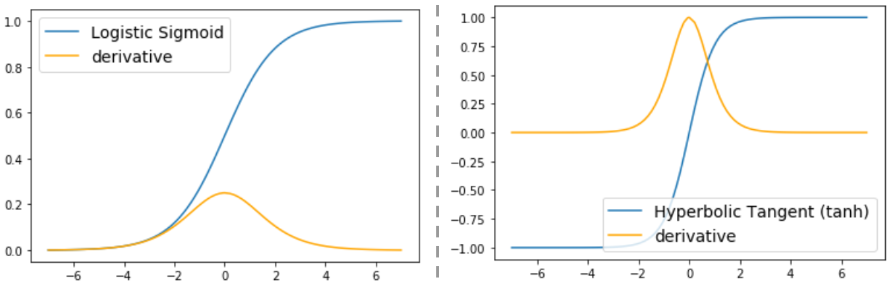
\includegraphics{figure/derivs_sigm_tanh.png}}
      \caption{Sigmoidal activations (Savino \& Tondolo, 2021)}
    \end{figure}
    \item In each case, the function is only sensitive to its inputs in a small neighborhood around $0$.
    \item Furthermore, the derivative is never greater than 1 and is close to zero across much of the domain.
  \end{itemize}
\end{frame}

\begin{vbframe}{Sigmoidal Activation Functions}

\begin{enumerate}
  \item \textbf{Saturating Neurons:}
  \begin{itemize}
    \item We know: $\sigma'\left(z_{in}\right) \to 0$ for $|z_{in}| \to \infty$. 
    \item[$\to$] Neurons with sigmoidal activations "saturate" easily, that is, they stop being responsive when $|z_{in}| \gg 0$. 
  \end{itemize}

  \framebreak 

  \item \textbf{Vanishing Gradients: } Consider the vector of error signals $\bm{\delta}^{(i)}$ in layer $i$ 

    $$
      \bm{\delta}^{(i)} = \Wmat^{(i + 1)} \bm{\delta}^{(i + 1)} \odot \sigma'\left(\bm{z}_{in}^{(i)}\right), i \in\{ 1, ..., O\}. 
    $$

    Each $k$-th component of the vector expresses how much the loss $L$ changes when the input to the $k$-th neuron $z_{k, in}^{(i)}$ changes. 
    \begin{itemize}
      \item We know: $\sigma'(z)< 1$ for all $z \in \mathbb{R}$. 
      \item[$\to$] In each step of the recursive formula above, the value will be multiplied by a value smaller than one
      \begin{eqnarray*}
        \bm{\delta}^{(1)} &=& \Wmat^{(2)} \bm{\delta}^{(2)} \odot \sigma'\left(z_{in}^{(i)}\right) \\
        &=& \Wmat^{(2)} \left(\Wmat^{(3)} \bm{\delta}^{(3)} \odot \sigma'\left(z_{in}^{(i)}\right)\right) \odot \sigma'\left(z_{in}^{(i)}\right) \\
        &=& ...
      \end{eqnarray*}
      \item When this occurs, earlier layers train \emph{very} slowly (or not at all).
    \end{itemize}
\end{enumerate}

\end{vbframe}


\begin{frame} {Rectified Linear Units (ReLU)}
  \begin{itemize}
    \item The ReLU activation solves the vanishing gradient problem.
    \begin{figure}
      \centering
        \scalebox{1}{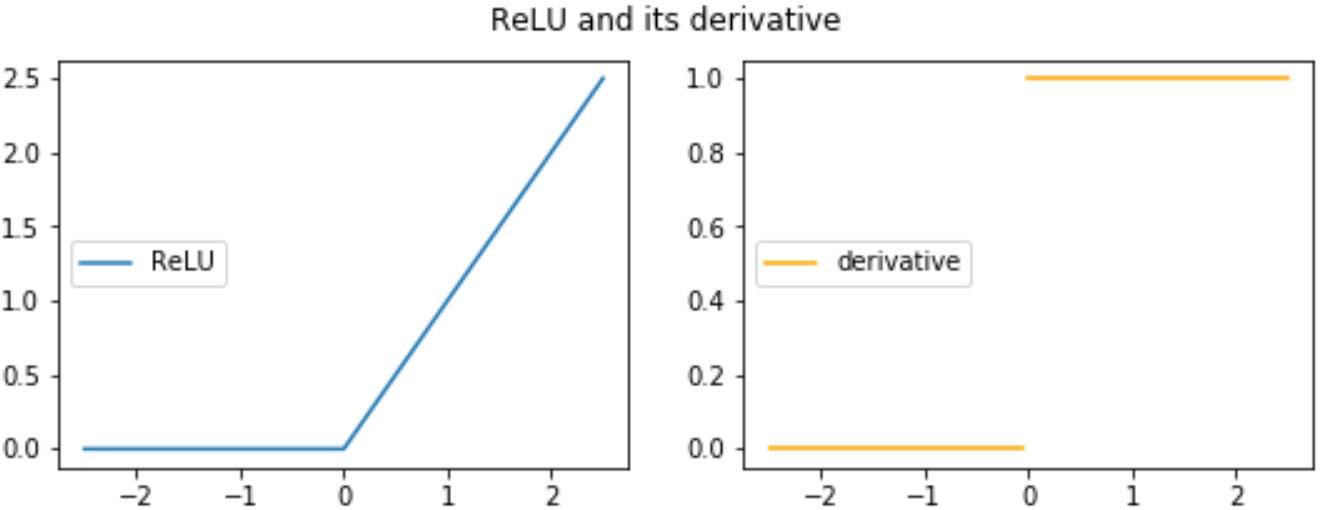
\includegraphics{figure/relu_deriv.png}}
        \caption{ReLU activation (Savino \& Tondolo, 2021)}
    \end{figure}
    \item In regions where the activation is positive, the derivative is $1$. 
    \item As a result, the derivatives do not vanish along paths that contain such "active" neurons even if the network is deep.
    \item Note that the ReLU is not differentiable at 0 (Software implementations return either $0$ or $1$ for the derivative at this point).
  \end{itemize}
\end{frame}

\begin{frame} {Rectified Linear Units (ReLU)}
  \begin{itemize}
    \item ReLU units can significantly speed up training compared to units with saturating activations.
    \begin{figure}
    \centering
      \scalebox{0.65}{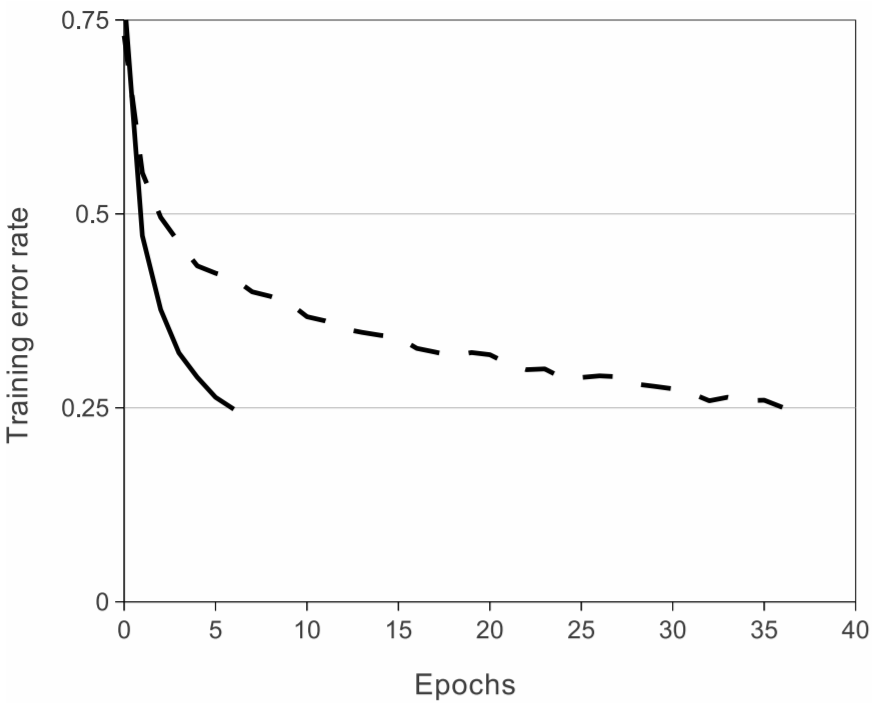
\includegraphics{figure/relu_vs_tanh.png}}
      \caption{\footnotesize A four-layer convolutional neural network with ReLUs (solid line) reaches a 25\% 
training error rate on the CIFAR-10 dataset six times faster than an equivalent network with tanh neurons (dashed line) (Krizhevsky et al., 2012). }
    \end{figure}
  \end{itemize}
\end{frame}

\begin{frame} {Rectified Linear Units (ReLU)}
  \begin{itemize}
  \item A downside of ReLU units is that when the input to the activation is negative, the derivative is zero. This is known as the "dying ReLU problem".
    \begin{figure}
      \centering
        \scalebox{1}{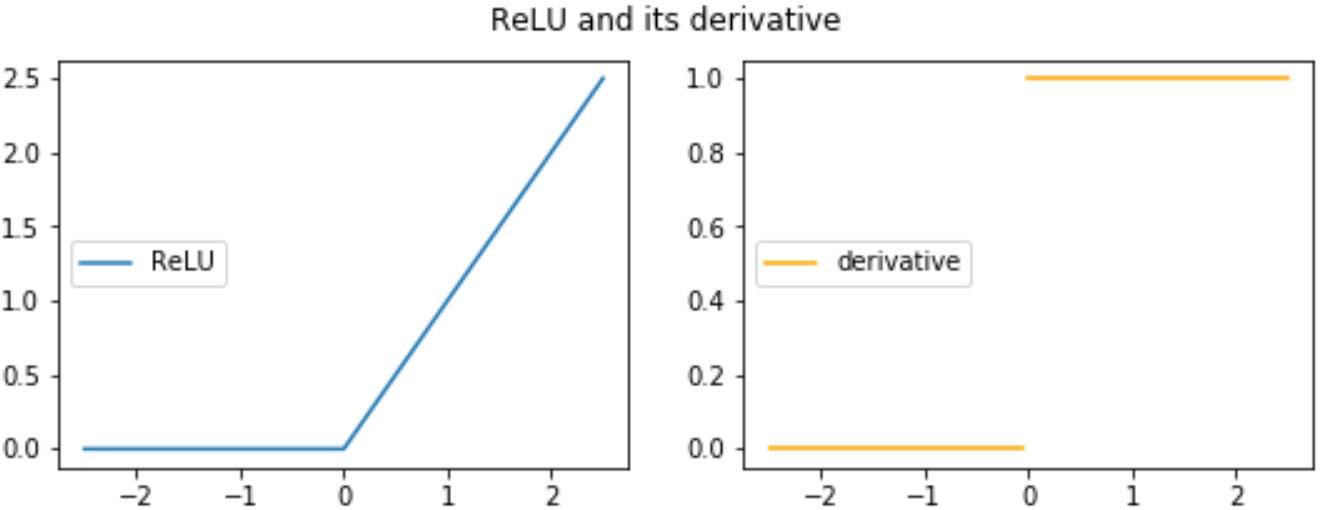
\includegraphics{figure/relu_deriv.png}}
        \caption{ReLU activation (Savino \& Tondolo, 2021)}
    \end{figure}
    \item When a ReLU unit "dies", that is, when its activation is 0 for all datapoints, it kills the gradient flowing through it during backpropogation.
    \item This means such units are never updated during training and the problem can be irreversible.
   
  \end{itemize}
\end{frame}

\begin{frame} {Generalizations of ReLU}
  \begin{itemize}
    \item There exist several generalizations of the ReLU activation that have non-zero derivatives throughout their domains.
    \item \emph{Leaky ReLU}: 
    $$  LReLU(v) = \begin{cases} 
          v & v \geq 0 \\
          \alpha v & v < 0 
       \end{cases} $$
    \begin{figure}
      \centering
        \scalebox{0.45}{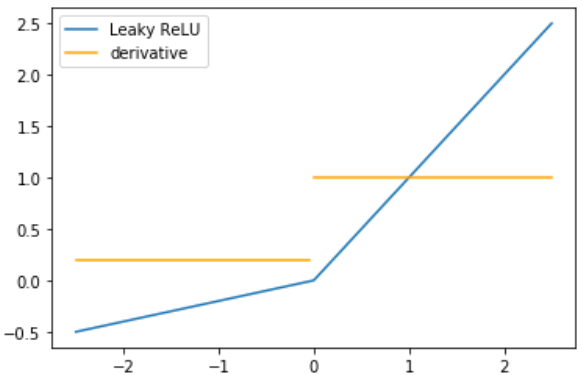
\includegraphics{figure/leakyrelu_deriv.png}}
        \caption{Leaky ReLU (Savino \& Tondolo, 2021)}
    \end{figure}
    \item Unlike the ReLU, when the input to the Leaky ReLU activation is negative, the derivative is $\alpha$ which is a small positive value (such as $0.01$).
  \end{itemize}
\end{frame}

\begin{frame} {Generalizations of ReLU}
  \begin{itemize}
    \item A variant of the Leaky ReLU is the \emph{Parametric ReLU (PReLU)} which learns the $\alpha$ from the data through backpropagation.

    \item \emph{Exponential Linear Unit (ELU)}:
    
    $$ ELU(v) = \begin{cases} 
          v & v \geq 0 \\
          \alpha (e^v - 1) & v < 0 
       \end{cases} $$

    \item \emph{Scaled Exponential Linear Unit (SELU)}:
    
    $$ SELU(v) = \lambda \begin{cases} 
          v & v \geq 0 \\
          \alpha (e^v - 1) & v < 0 
       \end{cases} $$
  
  {\scriptsize Note: In ELU and SELU, $\alpha$ and $\lambda$ are hyperparameters that are set before training.}
  \item These generalizations may perform as well as or better than the ReLU on some tasks. 
  \end{itemize}

\end{frame}

\begin{frame} {Generalizations of ReLU}
  \lz
  \lz
  \begin{figure}
    \centering
      \scalebox{1}{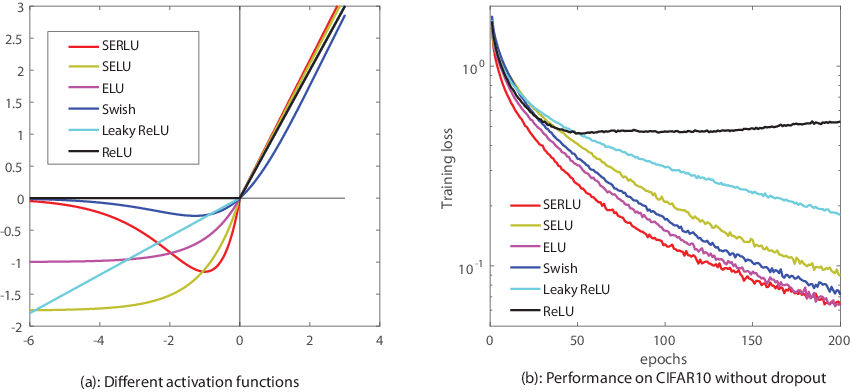
\includegraphics{figure/actfun_comparison.png}}
      \caption{Visualization of different generalisations of ReLU (Zhang et al., 2018)}
      \end{figure}
\end{frame}

% \begin{frame} {Hidden activations}
%   \begin{itemize}
%     \item In general, the design of activation functions is heuristically motivated.
%     \item Choice of hidden units doesn't make many guiding principles.
%     \item Difficult to predict a priori which ones
%     \item Aside from the ones we've seen, it is possible for many other functions to have comparable performance.
%     \item For example, 
%   \end{itemize}
% \end{frame}

\section{Output activations}

\begin{frame} {Output Activations}
  \begin{itemize}
    \item As we have seen previously, the role of the output activation is to get the final score on the same scale as the target.
    \item The output activations and the loss functions used to train neural networks can be viewed through the lens of maximum likelihood estimation (MLE).
    \item In general, the function $f(\xv~|~\thetab)$ represented by the neural network defines the conditional $p(y~|~\xv,\thetab)$ in a supervised learning task.
    \item Maximizing the likelihood is then equivalent to minimizing $- \log p(y~|~\xv,\thetab)$.
    \item An output unit with the identity function as the activation can be used to represent the mean of a Gaussian distribution.
    \item For such a unit, training with mean-squared error is equivalent to maximizing the log-likelihood (ignoring issues with non-convexity).
  \end{itemize}
\end{frame}


\begin{frame} {Output Activations}
  \begin{itemize}
    \item Similarly, sigmoid and softmax units can output the parameter(s) of a Bernoulli distribution and Categorical distribution, respectively.
    \item It is straightforward to show that when the label is one-hot encoded, training with the cross-entropy loss is equivalent to maximizing log-likelihood. \href{https://www.quora.com/What-are-the-differences-between-maximum-likelihood-and-cross-entropy-as-a-loss-function}{\beamergotobutton{Click here}}

    \item Because these activations can saturate, an important advantage of maximizing log-likelihood is that the $\log$ undoes some of the exponentiation in the activation functions which is desirable when optimizing with gradient-based methods.
    \item For example, in the case of softmax, the loss is:
    $$ L(y, \fx) = - f_{in,k} + \log {\sum_{k'=1}^g\exp(f_{in,k'})}$$ where $k$ is the correct class. The first term, $- f_{in,k}$, does not saturate which means training can progress steadily even if the contribution of $f_{in,k}$ to the second term is negligible.
  \end{itemize}
\end{frame}

\begin{frame} {Output Activations}
  \begin{itemize}
    \item A neural network can even be used to output the parameters of more complex distributions.
    \item A Mixture Density Network, for example, outputs the parameters of a Gaussian Mixture Model:
$$p(y | \xv)=\sum_{c=1}^{m} \phi^{(c)} (\xv) ~ \mathcal{N}\left(y ; \boldsymbol{\mu}^{(c)}(\xv), \boldsymbol{\Sigma}^{(c)}(\xv)\right)$$
          where $m$ the number of components in the mixture.
    \item In such a network, the output units are divided into groups.
    \item One group of output neurons with softmax activation represents the weights ($\phi^{(c)}$) of the mixture.
    \item Another group with the identity activation represents the means ($\boldsymbol{\mu}^{(c)}$) and yet another group with a non-negative activation function (such as ReLU or the exponential function) can represent the variances of the (typically) diagonal covariance matrices $\boldsymbol{\Sigma}^{(c)}$.
  \end{itemize}
\end{frame}

\begin{frame} {Output Activations}
  \begin{figure}
    \centering
      \scalebox{1}{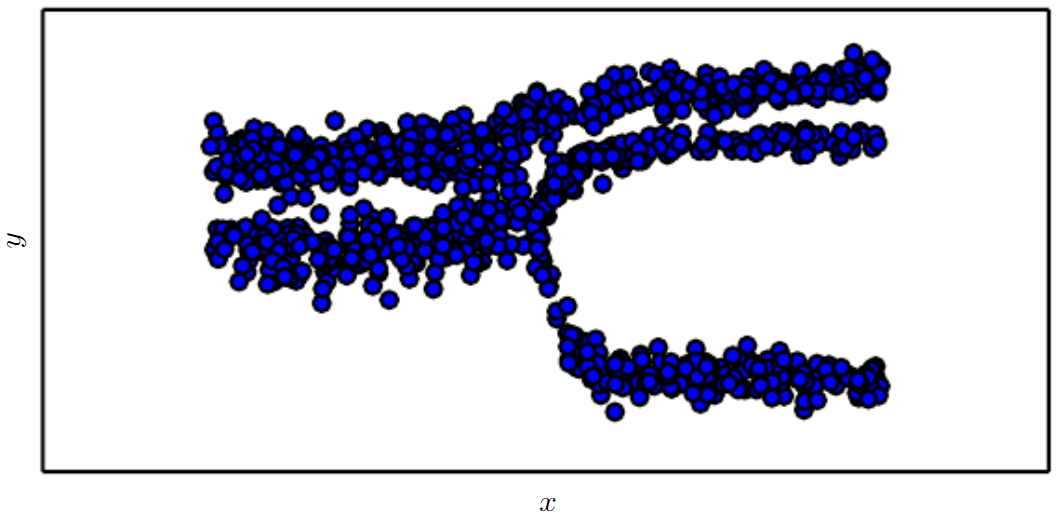
\includegraphics{figure/mdn.png}}
      \caption{\footnotesize Samples drawn from a Mixture Density Network. The input $\xv$ is sampled from a uniform distribution and $y$ is sampled from $p(y~|~\xv,\thetab)$ (Goodfellow et al., 2016).}
  \end{figure}
\end{frame}

%%%%%%%%%%%%%%%%%%%%%%%%%%%%%%%%%%%%%%%%%%%%%%%%%%%%%%%%%%%%%%%%%%
%%%%%%%%%%%%%%%%%%          REFERENCES          %%%%%%%%%%%%%%%%%%
%%%%%%%%%%%%%%%%%%%%%%%%%%%%%%%%%%%%%%%%%%%%%%%%%%%%%%%%%%%%%%%%%%
\begin{vbframe}
\frametitle{References}
\footnotesize{
\begin{thebibliography}{99}
%%%%%%%%%%%%%%%%%%%%%%%%%%%%%%%%%%
\bibitem[(Savino \& Tondolo, 2021)]{1}Savino, P., \& Tondolo, F. (2021). Automated classification of civil structure defects based on convolutional neural network. \textit{Frontiers of Structural and Civil Engineering, 15}(2), 305–317. \url{https://doi.org/10.1007/s11709-021-0725-9}


\bibitem[Ian Goodfellow et al., 2016]{1} 
Goodfellow, I., Bengio, Y., \& Courville, A. (2016). \textit{Deep Learning}. MIT Press.

%%%%%%%%%%%%%%%%%%%%%%%%%%%%%%%%%%
\bibitem[(Krizhevsky et al., 2012)]{1} 
Krizhevsky, A., Sutskever, I., \& Hinton, G. E. (2012). ImageNet Classification with Deep Convolutional Neural Networks. In F. Pereira, C. J. Burges, L. Bottou, \& K. Q. Weinberger (Eds.), \textit{Advances in Neural Information Processing Systems} (Vol. 25). Curran Associates, Inc. \url{https://proceedings.neurips.cc/paper_files/paper/2012/file/c399862d3b9d6b76c8436e924a68c45b-Paper.pdf}

%%%%%%%%%%%%%%%%%%%%%%%%%%%%%%%%%%
\bibitem[(Zhang et al., 2018)]{1}
Zhang, G., \& Li, H. (2018). \textit{Effectiveness of Scaled Exponentially-Regularized Linear Units (SERLUs)}.

\end{thebibliography}
}
\end{vbframe}
%%%%%%%%%%%%%%%%%%%%%%%%%%%%%%%%%%%%%%%%%%%%%%%%%%%%%%%%%%%%%%%%%%
%%%%%%%%%%%%%%%%%%%%%%%%%%%%%%%%%%%%%%%%%%%%%%%%%%%%%%%%%%%%%%%%%%

\endlecture
\end{document}